\section{Simulation Framework Benchmarking}
\label{sec:results-part1-runtime-scaling}

This section benchmarks the computational viability of our integrated simulation framework. Specifically, we evaluate the cost of replacing the standard stochastic ns-3 propagation model with the deterministic Sionna RT engine embedded directly within the simulator process.
To establish a baseline for our framework's efficiency, we compare three distinct channel backends: \texttt{pure ns-3}, \texttt{ns3sionna}, and our embedded \texttt{sionnart} module.
The \texttt{pure ns-3} backend utilizes the conventional ns-3 stochastic propagation model,
while the \texttt{ns3sionna} \cite{ns3sionna} implementation relies on communicating with an external Python-based Sionna RT server via ZMQ sockets.
Finally, \texttt{sionnart} runs Sionna RT directly inside the simulator's address space using pybind11 \cite{sionna,sionnart,pybind11}.
To benchmark the computational cost of the three channel backends, the same network topology — a single IEEE 802.11ax access point and $N\in\{1,2,4,8,16,32\}$ stations — and the same application traffic profile are used.
The benchmarking is done on IEEE 802.11ax instead of 5G NR as the \texttt{ns3sionna} \cite{ns3sionna} is tested only on IEEE 802.11ax and not on 5G NR.
Keeping topology and traffic fixed ensures that runtime differences are caused solely by the channel backend.
With the same setup, three different scenarios are simulated:
\begin{itemize}
    \item \textbf{stationary\_high\_load}: static nodes and high packet rate;
    \item \textbf{low\_mob\_low\_load}: slow random-walk mobility and low packet rate;
    \item \textbf{high\_mob\_high\_load}: fast random-walk mobility and high packet rate.
\end{itemize}
The last scenario is to stress test the ray tracing because mobility repeatedly invalidates the cache of channels while the high packet rate keeps the simulator issuing propagation queries.

\subsubsection{Total Simulation Time Scaling}
\label{subsec:total-sim-time-scaling}

Figure \ref{fig:total-sim-time-scaling} shows the total time taken to finish the simulation over the number of stations $N$ with different channel backends.
The y-axis is in logarithmic scale because the total simulation time spans more than four orders of magnitude between the smallest and largest runs.
The same results are presented in Table \ref{tab:total-sim-time-scaling}.
\begin{figure}[t]
    \centering
    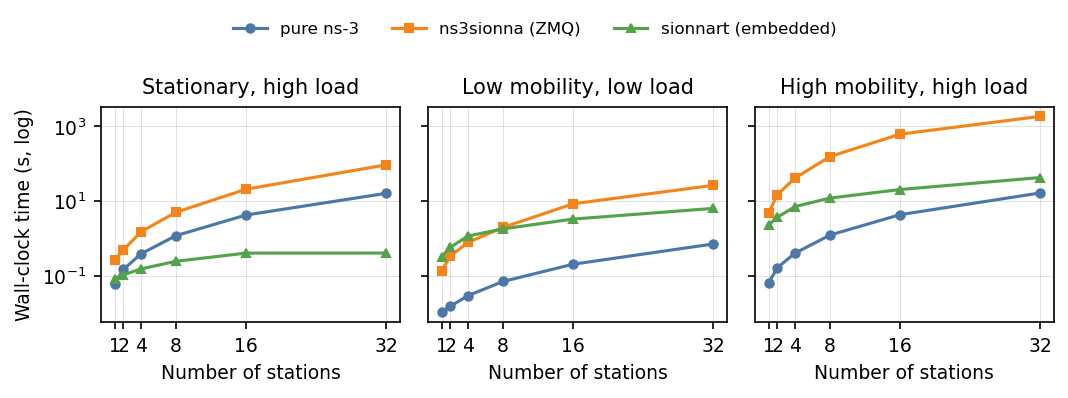
\includegraphics[width=\linewidth]{images/total-sim-time-scaling.png}
    \caption{Total simulation runtime of the three channel backends as the number of
        stations increases. The communication with external Sionna RT server via ZMQ in \texttt{ns3sionna} causes large overhead.
        The embedded \texttt{sionnart} backend avoids the round trip overhead, while the pure ns-3 baseline
        provides the analytical-channel lower bound.}
    \label{fig:total-sim-time-scaling}
\end{figure}

\begin{table}[t]
    \centering
    \caption{Total simulation runtime in seconds for representative station counts.}
    \label{tab:total-sim-time-scaling}
    \setlength{\tabcolsep}{5pt}
    \begin{tabular}{llrrrr}
        \hline
        Regime        & Backend   & $N=1$ & $N=4$  & $N=16$  & $N=32$   \\
        \hline
        Stationary    & pure ns-3 & 0.061 & 0.385  & 4.230   & 16.160   \\
        Stationary    & ns3sionna & 0.266 & 1.504  & 20.826  & 93.834   \\
        Stationary    & sionnart  & 0.082 & 0.152  & 0.403   & 0.404    \\
        \hline
        Low mobility  & pure ns-3 & 0.010 & 0.029  & 0.203   & 0.708    \\
        Low mobility  & ns3sionna & 0.137 & 0.778  & 8.453   & 26.439   \\
        Low mobility  & sionnart  & 0.320 & 1.153  & 3.292   & 6.370    \\
        \hline
        High mobility & pure ns-3 & 0.064 & 0.400  & 4.320   & 16.516   \\
        High mobility & ns3sionna & 4.821 & 41.312 & 622.365 & 1871.600 \\
        High mobility & sionnart  & 2.293 & 7.124  & 20.405  & 42.772   \\
        \hline
    \end{tabular}
\end{table}

The scaling behavior of time taken for simulation differs across different scenarios.
In the stationary scenario, the apparent advantage of \texttt{sionnart} over the \texttt{pure\_ns-3} baseline is an artefact of the cache (Section~\ref{subsec:cache-validity}), not evidence that ray-tracing is intrinsically faster than Friis evaluation.
Because no UE moves, the ray-tracer is invoked only once at $t=0$; all subsequent propagation queries are served from the cached channel snapshot while the analytical baseline still re-evaluates its loss model at every packet arrival.
This cache-driven effect produces an approximately $40\times$ wall-clock reduction at $N=32$, and would collapse to a significant overhead if mobility were introduced without the cache.
Even in this stationary scenario, \texttt{ns3sionna} backend is slower than both \texttt{pure\_ns-3} and \texttt{sionnart} backends due to the overhead of the communication between ns-3 and Sionna RT server.

In low-mobility, low-load scenario, the results show the opposite trade-off.
When the number of station counts ($N$) are low, \texttt{sionnart} is slower than \texttt{ns3sionna} because there are few propagation queries so that the cost of the query outweight the fixed cost of the embedded Python runtime and Sionna scene.
As $N$ grows, batching and cache reuse become more effective so that by the $N=32$ the performance of \texttt{sionnart} is 4.15 times faster than \texttt{ns3sionna}.
It remains 9 times slower than the \texttt{pure\_ns-3} baseline because the traffic load is low enough that stochastic propagation model remains cheap in term of computation.

The high-mobility, high-load scenario is the most important one because it is the most realistic scenario for the next generation wireless network.
In this scenario, \texttt{ns3sionna} scales poorly with the number of stations because each cache misses require copying data between processes, waiting for a request and response between two servers, and updating the Sionna side state.
The \texttt{sionnart} backend still have to pay the price of invoking the ray-tracer for each cache miss, but it avoid the overhead of inter-process communication and keeps the cache inside the same process.
As a result, the gap between \texttt{sionnart} and \texttt{ns3sionna}  grows monotonically from 2.1 times at $N=1$ to 43.8 times at $N=32$.


\subsubsection{Speedup Analysis}
\label{subsec:speedup-analysis}
Figire \ref{fig:speed-comparison} shows the runtime ratios.
The left panel shows $T_{\mathrm{ns3sionna}}/T_{\mathrm{sionnart}}$ and a larger value means that \texttt{sionnart} is faster than \texttt{ns3sionna}.
The right panel shows $T_{\mathrm{sionnart}}/T_{\mathrm{pure\ ns3}}$ and a value below one means that \texttt{sionnart} is faster than \texttt{pure\_ns-3} baseline.
The same results are show in Table \ref{tab:speed-comparison}.

\begin{figure}[t]
    \centering
    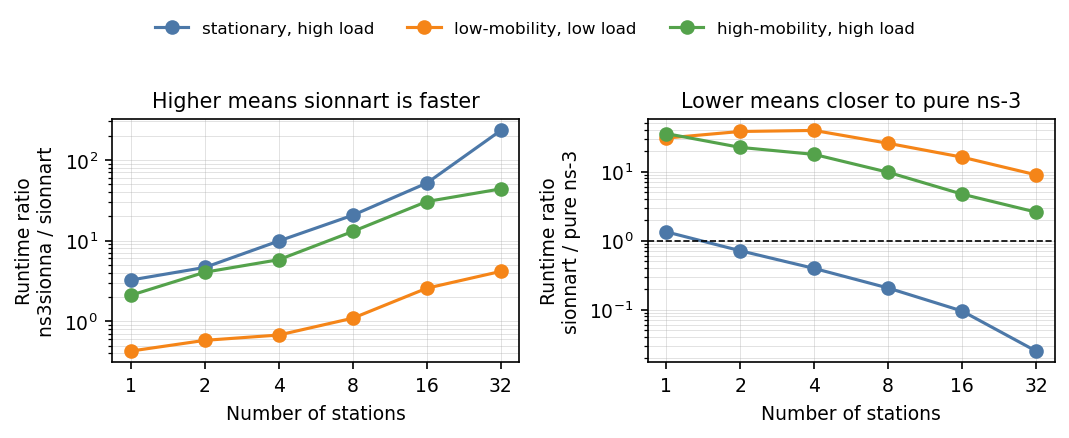
\includegraphics[width=\linewidth]{images/speed_comparison.png}
    \caption{The left graph shows the ratio of \texttt{ns3sionna} runtime to \texttt{sionnart} runtime.
        The right graph is the ratio of \texttt{sionnart} runtime to \texttt{pure\_ns-3} baseline runtime.}
    \label{fig:speed-comparison}
\end{figure}

According to these ratios, embedding Sionna RT using pybind11 helps to improve the performance of simulation.
In two server design, a cache miss must send data from ns-3 to a separate Python process and wait for the reply.
In the embedded design, ns-3, the cache, Sionna RT, all run inside the same process.
This removes much of the communication cost and the remaining cost is the actual ray-tracing, which is still needed when the experiment uses site-specific propagation.

\begin{table}[t]
    \centering
    \caption{Ratios at $N=32$. The first ratio is
    $T_{\mathrm{ns3sionna}}/T_{\mathrm{sionnart}}$; the second is
    $T_{\mathrm{sionnart}}/T_{\mathrm{pure\ ns3}}$.}
    \label{tab:speed-comparison}
    \setlength{\tabcolsep}{5pt}
    \begin{tabular}{lrr}
        \hline
        Scenario                 & Speedup over  & Cost relative \\
                                 & ns3sionna     & to pure ns-3  \\
        \hline
        Stationary, high load    & $232.3\times$ & $0.025\times$ \\
        Low mobility, low load   & $4.15\times$  & $9.00\times$  \\
        High mobility, high load & $43.8\times$  & $2.59\times$  \\
        \hline
    \end{tabular}
\end{table}

However, two server design is also have its own merits.
Having separate server for Sionna RT allows us to run the ray-tracing engine on a different machine, and it also allows us to run multiple ray-tracing engines in parallel.
But for our use case, we only need to run the ray-tracing engine on the same machine as ns-3.
So we choose the embedded design.

\subsubsection{GPU Footprint and Utilization}
\label{subsec:gpu-usage}

Figure \ref{fig:gpu-usage} shows the GPU memory footprint and processing core utilization for each scenario.
For \texttt{sionnart}, allocated memory is almost flat.
It is $337$ MiB for the smallest stationary scenario, about $465$-$469$ MiB for most scenarios, and $491$ MiB for the largest high-mobility scenario.
This is because most of the memory usage is due to the Sionna RT scene and increasing number of stations in the same scene, not the number of packets processed by ns-3.
By contrast, \texttt{ns3sionna} grows significantly in the high-mobility scenario.
The memory increases from $730$ MiB at $N=1$ to $7858$ MiB at $N=32$.

\begin{figure}[t]
    \centering
    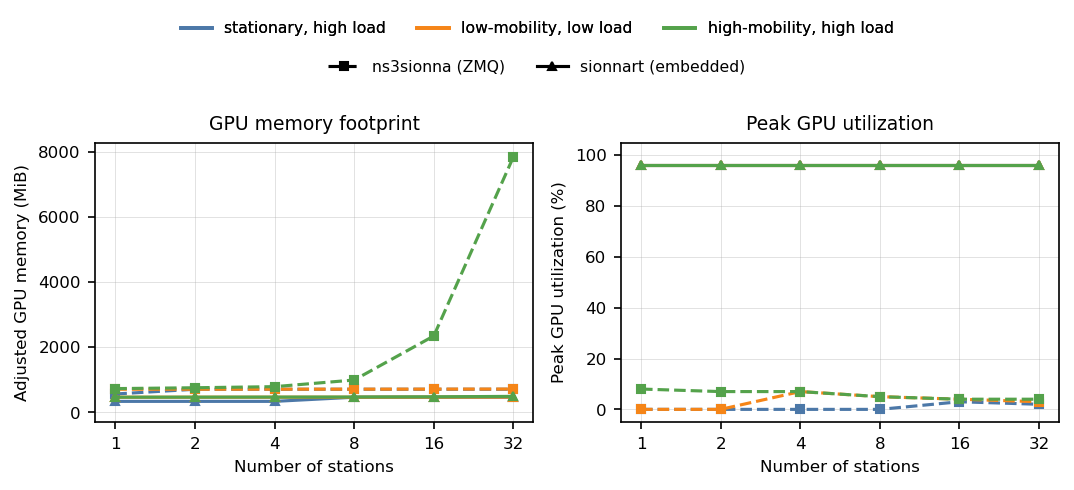
\includegraphics[width=\linewidth]{images/gpu_usage.png}
    \caption{Reported GPU memory footprint and peak utilization for the two
        Sionna-backed backends.}
    \label{fig:gpu-usage}
\end{figure}

The peak-utilization panel present the maximum observed value but not the average GPU load.
\texttt{sionnart} utilize upto $96\%$ at its peak for performing the channel calculations but the duration of running at peak is very short.
On the other hand, \texttt{ns3sionna} has lower peak utilization but the GPU is busy most of the time.

In summary, \texttt{sionnart} keeps a nearly fixed GPU memory footprint because the scene and others are reused across channel queries.
\texttt{ns3sionna} uses much more memory because it has to keep per-link ray-tracing state as the number of mobile links increases.
For \texttt{sionnart}, it utilize full potential of GPU and duration of running calculation is very short while the \texttt{ns3sionna} is busy most of the time with lower peak utilization.
